\chapter{Parameter Estimation}
Given a decision rule, $U(x,w)$, the unknown parameter $w$ need to be estimated. This is unique to frequentist statistics as the parameters $w$ are considered realizations of random variables in Bayesian statistics. $w$ is estimated by re-applying decision theory. To distinguish this scenario from previous ones, denote the decision rule in this case $\hat{w}$.


\begin{definition}[Fisher Information]
	\label{def:fisher_information}
	The Fisher information is a way of measuring the amount of information about an unknown parameter a random variable contains. Let $w$ be an unknown parameter, $p(X|w)$ a probability distribution for the generic random variable $X:\Omega\mapsto \Omega_X$ and define $l(X|w,I)= \frac{\partial}{\partial w} \ln p(X|w,I)$. The Fisher information can then be written
	\begin{equation}
		\begin{split}
			\mathcal{I}(w) &\equiv \mathbb{E} [l(X|w)^2|w,I]\\
			&= \operatorname{Var}[l(X|w)|w,I].
		\end{split}
	\end{equation}
\end{definition}

\begin{proof}
	In general 
	\begin{equation}
		\mathbb{E} [l(X|w)^2|w,I] = \operatorname{Var}[l(X|w)|w,I]+\mathbb{E}[l(X|w)|w,I]^2
	\end{equation}
	however
	\begin{equation}
		\begin{split}
			\mathbb{E}[l(X|w,I)|w] &= \int  \frac{\partial}{\partial w} \ln p(X=x|w,I) p(X=x|w,I) dx\\
			&= \frac{\partial}{\partial w}\int  p(X=x|w,I) dx\\
			&= 0.\\
		\end{split}
	\end{equation}
\end{proof}


\begin{theorem}[Fisher information for sample]
	Let $X_1,X_2,\dots X_n$ be a set of independent and identically distributed random variables from the measurable space $(\Omega,\mathcal{F})$. The Fisher information in a sample is 
	\begin{equation}
		\mathcal{I}(w) = n\mathcal{I}_1(w),
	\end{equation}
	where $\mathcal{I}_1(w)$ is the Fisher information of any one of the random variables.
\end{theorem}


\begin{definition}[Maximum Likelihood Estimator (MLE) Decision Rule]
	\label{def:MLE}
	The Maximum Likelihood Estimator (MLE) decision rule $\hat{w}_{\text{MLE}}$ is defined as the decision rule that maximizes the likelihood $p(D_s|D_x,w)$ given the data $D_x$ and past Nature decisions $D_s$
	\begin{equation}
		\hat{w}_{\text{MLE}}(\tilde{D}) \equiv \arg \max_{w} p(D_s|D_x,w,I).
	\end{equation}
\end{definition}

\begin{theorem}[Unbiasedness of the MLE Decision Rule]
	\label{thm:unbiased_mle}
	Under certain regularity conditions, the MLE decision rule $\hat{w}_{\text{MLE}}$ is asymptotically unbiased, meaning
	\begin{equation}
		\sqrt{n}(\hat{w}_{\text{MLE}}-w)\xrightarrow[]{\text{d}} N(0,I(w)^{-1}),
	\end{equation}
	where $I(w)^{-1}$ is the Fisher information matrix at $w$ and $\xrightarrow[]{\text{d}}$ represents convergence in distribution.
\end{theorem}

\begin{definition}[Minimax Decision Rule]
	\label{def:minimax}
	A decision rule $\hat{w}'$ is said to be minimax if it minimize the maximum expected cost, meaning
	\begin{equation}
		\hat{w}' \equiv \inf_{\hat{w}}\sup_{w\in \Omega_W}\mathbb{E}[C(\hat{w},w)|w,D,I].
	\end{equation}
\end{definition}

\begin{theorem}[Mean Squared Error (MSE)]
	\label{theorem:MSE}
	The expectation of the quadratic cost function (\dfref{def:quadratic_cost}) can be written
	\begin{equation}
		\begin{split}
			\mathbb{E}[C(\hat{w}, w)|w,D,I] &= \mathbb{E}[(\hat{w}-w)^2|w,D,I]\\ 
			&= \mathbb{E}[(\hat{w}-\mathbb{E}[\hat{w}])^2]+(w-\mathbb{E}[\hat{w}])^2\\
			&=\operatorname{Var}[\hat{w}]+\text{Bias}[\hat{w}]^2\\
		\end{split}
		\label{eq:MSE}
	\end{equation}
	where conditions have been suppressed in the second line (to fit to the page) and the bias of the estimator of $\hat{w}$ is defined viz
	\begin{equation}
		\text{Bias}[\hat{w}]\equiv w-\mathbb{E}[\hat{w}|w,D,I].
	\end{equation}
	If $\mathbb{E}[C(\hat{w}, w)|w,D,I]\xrightarrow[]{\text{data}\rightarrow\infty} 0$ then $C(\hat{w}, w)$ is a weakly consistent estimate of $w$. There can be different consistent estimates that converge towards $w$ at different speeds. It is desirable for an estimate to be consistent and with small (quadratic) cost, meaning that both the bias and variance of the estimator should be small. In many cases, however, there is bias-variance which means that both cannot be minimized at the same time. 
\end{theorem}

\begin{corollary}[MLE is Approximately Minimax for quadratic Loss]
	\label{cor:MLE_minimax}
	Under certain regularity conditions, the Maximum Likelihood decision rule (MLE) $\hat{w}_{\text{MLE}}$ is approximately minimax for the quadratic cost function (\dfref{def:quadratic_cost}), meaning it approximately minimizes the maximum expected cost.
	
	\begin{proof}
		From theorem \thref{theorem:MSE}
		\begin{equation}
			\mathbb{E}[(\hat{w}-w)^2] = \operatorname{Var}[\hat{w}]+\text{Bias}[\hat{w}]^2.
		\end{equation}
		Under the regularity conditions where the MLE is unbiased and has asymptotically minimal variance, the bias term vanish, meaning $\text{Bias}[\hat{w}_{\text{MLE}}] = 0$ and the variance term $\operatorname{Var}[\hat{w}_{\text{MLE}}]$ is minimized among a class of estimators. Thus, the expected quadratic cost for the MLE can be approximated by
		\begin{equation}
			\begin{split}
				\mathbb{E}[(\hat{w}_{\text{MLE}}-w)^2] &\approx \operatorname{Var}[\hat{w}_{\text{MLE}}]\\
				&\approx \frac{\text{tr}[I(w)^{-1}]}{n},
			\end{split}
		\end{equation}
		where \thref{thm:unbiased_mle} was used for the second line. The Cramer-Rao lower bound~\citep{Rao1973Linear} for variance states that 
		\begin{equation}
			\operatorname{Var}[\hat{w}]\geq \frac{\text{tr}[I(w)^{-1}]}{n},
		\end{equation}
		implying that the MLE decision rule acheives the smallest possible variance asymptotically and therefore that 
		\begin{equation}
			\sup_{w\in \Omega_W}\mathbb{E}[(\hat{w}_{\text{MLE}}-w)^2]\approx \inf_{\hat{w}} \sup_{w \in \Omega_W} \mathbb{E}[(\hat{w} - w)^2],
		\end{equation}
		meaning the MLE decision rule is approximately the minimax decision rule under quadractic cost.
	\end{proof}
\end{corollary}

\begin{example}
	The bias-variance decomposition (\thref{theorem:MSE}) is only relevant for frequentist statistics and Bayesian statistics does not struggle with this tradeoff. It relates to overfitting and underfitting. Bayesians do not fit in the same way as frequentists do. They do not determine a single set of parameters, rather they use a set of parameters due to integration. In that sense, they are protected against overfitting and underfitting and they do not struggle with hyperparameter finetuning as well.
\end{example}

\begin{example}
	\emph{Consider $X_1,\dots, X_n\sim Ber(w)$. Determine the (quadratic) cost of three different decision rules for the mean; the arithmetic sample mean, the number $0.5$ and the first data entry and $X_1$.}\newline
	
	\begin{itemize}
		\item For the arithmetic mean
		\begin{equation}
			\hat{w}=\frac{1}{n}\sum_{i=1}^nX_i
		\end{equation}
		meaning
		\begin{equation}
			\begin{split}
				\mathbb{E}[\hat{w}] & = \frac{1}{n}\sum_{i=1}^n\mathbb{E}[X_i]\\
				&=w,\\
				\operatorname{Var}[\hat{w}]	&= \frac{1}{n^2}\sum_{i=1}^n\operatorname{Var}[X_i]\\
				& = \frac{w(1-w)}{n},\\
				\mathbb{E}[(\hat{w}-w)^2]&=\frac{w(1-w)}{n}.
			\end{split} 
		\end{equation}

		\item For the number $0.5$ 
		\begin{equation}
			\hat{w}=0.5
		\end{equation}
		meaning
		\begin{equation}
			\begin{split}
				\mathbb{E}[\hat{w}] & = 0.5,\\
				\operatorname{Var}[\hat{w}]	&= 0,\\
				\mathbb{E}[(\hat{w}-w)^2]&=(0.5-w)^2.
			\end{split} 
		\end{equation}
		
		\item For the first entry, $X_1$,
		\begin{equation}
			\hat{w}=\frac{1}{n}\sum_{i=1}^nX_i
		\end{equation}
		meaning
		\begin{equation}
			\begin{split}
				\mathbb{E}[\hat{w}] & = \mathbb{E}[X_1]\\
				&=w,\\
				\operatorname{Var}[\hat{w}]	&= \operatorname{Var}[X_1]\\
				& = w(1-w),\\
				\mathbb{E}[(\hat{w}-w)^2]&=w(1-w).
			\end{split} 
		\end{equation}
	\end{itemize}
	The arithmetic mean minimizes the quadratic cost over the entire range of $w$, while the constant value $0.5$ performs better for a specific range of $w$. The cost for $X_1$ is independent of $n$, making it less favorable as $n$ increases.	
	\begin{figure}[H]
		\captionsetup{width=1\textwidth}
		\centering
		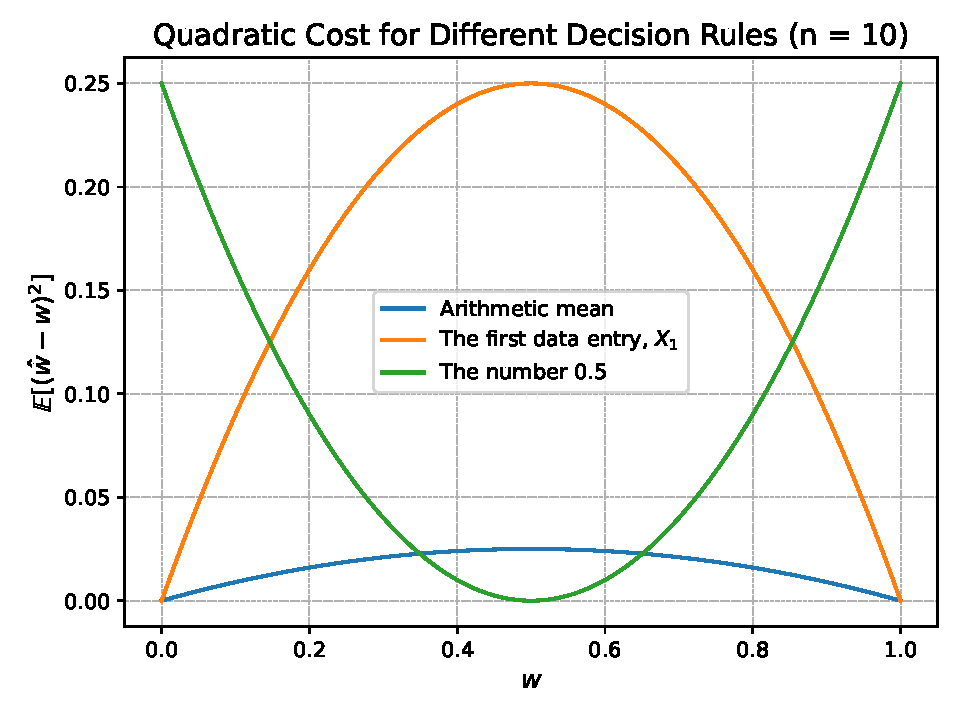
\includegraphics[width=1\textwidth]{figures/ber_example.pdf}
		\caption{The quadratic cost, $\mathbb{E}[(\hat{w} - w)^2]$, for three different decision rules: the arithmetic mean (blue), the first data entry $X_1$ (orange), and the constant value $0.5$ (green).}
		\label{fig:pen}
	\end{figure}
	
\end{example}

\begin{example}
	\emph{Determine the maximum likelihood estimate of $w$ for the model\newline $(\{0,1\},\{Ber(w)\}_{w\in(0,1)})$.}\newline
	
	\noindent In this case
	\begin{equation}
		\begin{split}
			p(D_s|D_x,w,I)=\prod_{i=1}^nw^{x_i}(1-w)^{1-x_i}.
		\end{split}
	\end{equation}
	Let $l(w)\equiv ln p(D_s|D_x,w,I)$, then
	\begin{equation}
		\begin{split}
			\argmax_wl(w) & = \argmax_wp(D_s|D_x,w,I)\\
			&= \argmax_w\ln \bigg(\prod_{i=1}^nw^{x_i}(1-w)^{1-x_i}\bigg)\\
			&=\argmax_w \bigg[\ln w\sum_{i=1}^nx_i + \ln(1-w)\sum_{i=1}^n(1-x_i)\bigg]
		\end{split}
	\end{equation}
	Now 
	\begin{equation}
		\frac{d}{dw}l(w)=\frac{\sum_{i=1}^nx_i}{w}-\frac{n-\sum_{i=1}^nx_i}{1-w}
	\end{equation}
	Requiring the derivative to vanish means the maximum likelihood estimate of $w$ is given by
	\begin{equation}
		\hat{w}_{\text{MLE}}=\frac{1}{n}\sum_{i=1}^nx_i.
	\end{equation}
\end{example}
\begin{example}
	\emph{Determine the maximum likelihood estimate of $w$ for the model\newline $([0,\infty),\{\text{Exp}(w)\}_{w>0})$.}\newline
	
	\noindent In this case
	\begin{equation}
		\begin{split}
			p(D_s|D_x,w,I)=\prod_{i=1}^nw e^{-w x_i}.
		\end{split}
	\end{equation}
	Let $l(w)\equiv ln p(D_s|D_x,w,I)$, then
	\begin{equation}
		\frac{d}{dw}l(w)=\frac{n}{w}-\sum_{i=1}^nx_i
	\end{equation}
	Requiring the derivative to vanish means the maximum likelihood estimate of $w$ is given by
	\begin{equation}
		\hat{w}_{\text{MLE}}=\frac{1}{\frac{1}{n}\sum_{i=1}^nx_i}.
	\end{equation}
\end{example}







